% Options for packages loaded elsewhere
% Options for packages loaded elsewhere
\PassOptionsToPackage{unicode}{hyperref}
\PassOptionsToPackage{hyphens}{url}
\PassOptionsToPackage{dvipsnames,svgnames,x11names}{xcolor}
\PassOptionsToPackage{space}{xeCJK}
%
\documentclass[
  chinese-hans,
  letterpaper,
  DIV=11,
  numbers=noendperiod]{scrartcl}
\usepackage{xcolor}
\usepackage{amsmath,amssymb}
\setcounter{secnumdepth}{5}
\usepackage{iftex}
\ifPDFTeX
  \usepackage[T1]{fontenc}
  \usepackage[utf8]{inputenc}
  \usepackage{textcomp} % provide euro and other symbols
\else % if luatex or xetex
  \usepackage{unicode-math} % this also loads fontspec
  \defaultfontfeatures{Scale=MatchLowercase}
  \defaultfontfeatures[\rmfamily]{Ligatures=TeX,Scale=1}
\fi
\usepackage{lmodern}
\ifPDFTeX\else
  % xetex/luatex font selection
  \ifXeTeX
    \usepackage{xeCJK}
    \setCJKmainfont[]{HarmonyOS Sans SC}
  \fi
  \ifLuaTeX
    \usepackage[]{luatexja-fontspec}
    \setmainjfont[]{HarmonyOS Sans SC}
  \fi
\fi
% Use upquote if available, for straight quotes in verbatim environments
\IfFileExists{upquote.sty}{\usepackage{upquote}}{}
\IfFileExists{microtype.sty}{% use microtype if available
  \usepackage[]{microtype}
  \UseMicrotypeSet[protrusion]{basicmath} % disable protrusion for tt fonts
}{}
\makeatletter
\@ifundefined{KOMAClassName}{% if non-KOMA class
  \IfFileExists{parskip.sty}{%
    \usepackage{parskip}
  }{% else
    \setlength{\parindent}{0pt}
    \setlength{\parskip}{6pt plus 2pt minus 1pt}}
}{% if KOMA class
  \KOMAoptions{parskip=half}}
\makeatother
% Make \paragraph and \subparagraph free-standing
\makeatletter
\ifx\paragraph\undefined\else
  \let\oldparagraph\paragraph
  \renewcommand{\paragraph}{
    \@ifstar
      \xxxParagraphStar
      \xxxParagraphNoStar
  }
  \newcommand{\xxxParagraphStar}[1]{\oldparagraph*{#1}\mbox{}}
  \newcommand{\xxxParagraphNoStar}[1]{\oldparagraph{#1}\mbox{}}
\fi
\ifx\subparagraph\undefined\else
  \let\oldsubparagraph\subparagraph
  \renewcommand{\subparagraph}{
    \@ifstar
      \xxxSubParagraphStar
      \xxxSubParagraphNoStar
  }
  \newcommand{\xxxSubParagraphStar}[1]{\oldsubparagraph*{#1}\mbox{}}
  \newcommand{\xxxSubParagraphNoStar}[1]{\oldsubparagraph{#1}\mbox{}}
\fi
\makeatother

\usepackage{color}
\usepackage{fancyvrb}
\newcommand{\VerbBar}{|}
\newcommand{\VERB}{\Verb[commandchars=\\\{\}]}
\DefineVerbatimEnvironment{Highlighting}{Verbatim}{commandchars=\\\{\}}
% Add ',fontsize=\small' for more characters per line
\usepackage{framed}
\definecolor{shadecolor}{RGB}{241,243,245}
\newenvironment{Shaded}{\begin{snugshade}}{\end{snugshade}}
\newcommand{\AlertTok}[1]{\textcolor[rgb]{0.68,0.00,0.00}{#1}}
\newcommand{\AnnotationTok}[1]{\textcolor[rgb]{0.37,0.37,0.37}{#1}}
\newcommand{\AttributeTok}[1]{\textcolor[rgb]{0.40,0.45,0.13}{#1}}
\newcommand{\BaseNTok}[1]{\textcolor[rgb]{0.68,0.00,0.00}{#1}}
\newcommand{\BuiltInTok}[1]{\textcolor[rgb]{0.00,0.23,0.31}{#1}}
\newcommand{\CharTok}[1]{\textcolor[rgb]{0.13,0.47,0.30}{#1}}
\newcommand{\CommentTok}[1]{\textcolor[rgb]{0.37,0.37,0.37}{#1}}
\newcommand{\CommentVarTok}[1]{\textcolor[rgb]{0.37,0.37,0.37}{\textit{#1}}}
\newcommand{\ConstantTok}[1]{\textcolor[rgb]{0.56,0.35,0.01}{#1}}
\newcommand{\ControlFlowTok}[1]{\textcolor[rgb]{0.00,0.23,0.31}{\textbf{#1}}}
\newcommand{\DataTypeTok}[1]{\textcolor[rgb]{0.68,0.00,0.00}{#1}}
\newcommand{\DecValTok}[1]{\textcolor[rgb]{0.68,0.00,0.00}{#1}}
\newcommand{\DocumentationTok}[1]{\textcolor[rgb]{0.37,0.37,0.37}{\textit{#1}}}
\newcommand{\ErrorTok}[1]{\textcolor[rgb]{0.68,0.00,0.00}{#1}}
\newcommand{\ExtensionTok}[1]{\textcolor[rgb]{0.00,0.23,0.31}{#1}}
\newcommand{\FloatTok}[1]{\textcolor[rgb]{0.68,0.00,0.00}{#1}}
\newcommand{\FunctionTok}[1]{\textcolor[rgb]{0.28,0.35,0.67}{#1}}
\newcommand{\ImportTok}[1]{\textcolor[rgb]{0.00,0.46,0.62}{#1}}
\newcommand{\InformationTok}[1]{\textcolor[rgb]{0.37,0.37,0.37}{#1}}
\newcommand{\KeywordTok}[1]{\textcolor[rgb]{0.00,0.23,0.31}{\textbf{#1}}}
\newcommand{\NormalTok}[1]{\textcolor[rgb]{0.00,0.23,0.31}{#1}}
\newcommand{\OperatorTok}[1]{\textcolor[rgb]{0.37,0.37,0.37}{#1}}
\newcommand{\OtherTok}[1]{\textcolor[rgb]{0.00,0.23,0.31}{#1}}
\newcommand{\PreprocessorTok}[1]{\textcolor[rgb]{0.68,0.00,0.00}{#1}}
\newcommand{\RegionMarkerTok}[1]{\textcolor[rgb]{0.00,0.23,0.31}{#1}}
\newcommand{\SpecialCharTok}[1]{\textcolor[rgb]{0.37,0.37,0.37}{#1}}
\newcommand{\SpecialStringTok}[1]{\textcolor[rgb]{0.13,0.47,0.30}{#1}}
\newcommand{\StringTok}[1]{\textcolor[rgb]{0.13,0.47,0.30}{#1}}
\newcommand{\VariableTok}[1]{\textcolor[rgb]{0.07,0.07,0.07}{#1}}
\newcommand{\VerbatimStringTok}[1]{\textcolor[rgb]{0.13,0.47,0.30}{#1}}
\newcommand{\WarningTok}[1]{\textcolor[rgb]{0.37,0.37,0.37}{\textit{#1}}}

\usepackage{longtable,booktabs,array}
\newcounter{none} % for unnumbered tables
\usepackage{calc} % for calculating minipage widths
% Correct order of tables after \paragraph or \subparagraph
\usepackage{etoolbox}
\makeatletter
\patchcmd\longtable{\par}{\if@noskipsec\mbox{}\fi\par}{}{}
\makeatother
% Allow footnotes in longtable head/foot
\IfFileExists{footnotehyper.sty}{\usepackage{footnotehyper}}{\usepackage{footnote}}
\makesavenoteenv{longtable}
\usepackage{graphicx}
\makeatletter
\newsavebox\pandoc@box
\newcommand*\pandocbounded[1]{% scales image to fit in text height/width
  \sbox\pandoc@box{#1}%
  \Gscale@div\@tempa{\textheight}{\dimexpr\ht\pandoc@box+\dp\pandoc@box\relax}%
  \Gscale@div\@tempb{\linewidth}{\wd\pandoc@box}%
  \ifdim\@tempb\p@<\@tempa\p@\let\@tempa\@tempb\fi% select the smaller of both
  \ifdim\@tempa\p@<\p@\scalebox{\@tempa}{\usebox\pandoc@box}%
  \else\usebox{\pandoc@box}%
  \fi%
}
% Set default figure placement to htbp
\def\fps@figure{htbp}
\makeatother



\ifLuaTeX
\usepackage[bidi=basic,shorthands=off,provide=*]{babel}
\else
\usepackage[bidi=default,shorthands=off,provide=*]{babel}
\fi
\ifLuaTeX
  \usepackage{selnolig} % disable illegal ligatures
\fi


\setlength{\emergencystretch}{3em} % prevent overfull lines

\providecommand{\tightlist}{%
  \setlength{\itemsep}{0pt}\setlength{\parskip}{0pt}}



 


\KOMAoption{captions}{tableheading}
\makeatletter
\@ifpackageloaded{tcolorbox}{}{\usepackage[skins,breakable]{tcolorbox}}
\@ifpackageloaded{fontawesome5}{}{\usepackage{fontawesome5}}
\definecolor{quarto-callout-color}{HTML}{909090}
\definecolor{quarto-callout-note-color}{HTML}{0758E5}
\definecolor{quarto-callout-important-color}{HTML}{CC1914}
\definecolor{quarto-callout-warning-color}{HTML}{EB9113}
\definecolor{quarto-callout-tip-color}{HTML}{00A047}
\definecolor{quarto-callout-caution-color}{HTML}{FC5300}
\definecolor{quarto-callout-color-frame}{HTML}{acacac}
\definecolor{quarto-callout-note-color-frame}{HTML}{4582ec}
\definecolor{quarto-callout-important-color-frame}{HTML}{d9534f}
\definecolor{quarto-callout-warning-color-frame}{HTML}{f0ad4e}
\definecolor{quarto-callout-tip-color-frame}{HTML}{02b875}
\definecolor{quarto-callout-caution-color-frame}{HTML}{fd7e14}
\makeatother
\makeatletter
\@ifpackageloaded{caption}{}{\usepackage{caption}}
\AtBeginDocument{%
\ifdefined\contentsname
  \renewcommand*\contentsname{目录}
\else
  \newcommand\contentsname{目录}
\fi
\ifdefined\listfigurename
  \renewcommand*\listfigurename{图索引}
\else
  \newcommand\listfigurename{图索引}
\fi
\ifdefined\listtablename
  \renewcommand*\listtablename{表索引}
\else
  \newcommand\listtablename{表索引}
\fi
\ifdefined\figurename
  \renewcommand*\figurename{图}
\else
  \newcommand\figurename{图}
\fi
\ifdefined\tablename
  \renewcommand*\tablename{表}
\else
  \newcommand\tablename{表}
\fi
}
\@ifpackageloaded{float}{}{\usepackage{float}}
\floatstyle{ruled}
\@ifundefined{c@chapter}{\newfloat{codelisting}{h}{lop}}{\newfloat{codelisting}{h}{lop}[chapter]}
\floatname{codelisting}{列表}
\newcommand*\listoflistings{\listof{codelisting}{列表索引}}
\makeatother
\makeatletter
\makeatother
\makeatletter
\@ifpackageloaded{caption}{}{\usepackage{caption}}
\@ifpackageloaded{subcaption}{}{\usepackage{subcaption}}
\makeatother
\usepackage{bookmark}
\IfFileExists{xurl.sty}{\usepackage{xurl}}{} % add URL line breaks if available
\urlstyle{same}
\hypersetup{
  pdftitle={皮尔逊相关分析},
  pdfauthor={Qingyao Zhang},
  pdflang={zh-Hans},
  colorlinks=true,
  linkcolor={blue},
  filecolor={Maroon},
  citecolor={Blue},
  urlcolor={Blue},
  pdfcreator={LaTeX via pandoc}}


\title{皮尔逊相关分析}
\usepackage{etoolbox}
\makeatletter
\providecommand{\subtitle}[1]{% add subtitle to \maketitle
  \apptocmd{\@title}{\par {\large #1 \par}}{}{}
}
\makeatother
\subtitle{Correlation}
\author{Qingyao Zhang}
\date{2026-04-13}
\begin{document}
\maketitle

\renewcommand*\contentsname{目录}
{
\setcounter{tocdepth}{3}
\tableofcontents
}

\begin{Shaded}
\begin{Highlighting}[numbers=left,,]
\FunctionTok{library}\NormalTok{(ggplot2)}
\FunctionTok{library}\NormalTok{(psych)}
\DocumentationTok{\#\# }
\DocumentationTok{\#\# Attaching package: \textquotesingle{}psych\textquotesingle{}}
\DocumentationTok{\#\# The following objects are masked from \textquotesingle{}package:ggplot2\textquotesingle{}:}
\DocumentationTok{\#\# }
\DocumentationTok{\#\#     \%+\%, alpha}
\FunctionTok{library}\NormalTok{(Keng)}
\FunctionTok{data}\NormalTok{(}\StringTok{"depress"}\NormalTok{, }\AttributeTok{package =} \StringTok{"Keng"}\NormalTok{)}
\end{Highlighting}
\end{Shaded}

\section{相关的概念}\label{ux76f8ux5173ux7684ux6982ux5ff5}

皮尔逊相关反映了两个变量之间的共变：

\begin{itemize}
\tightlist
\item
  X增加，Y便减少。
\item
  X增加，Y便增加。
\end{itemize}

\section{相关的三个特点}\label{ux76f8ux5173ux7684ux4e09ux4e2aux7279ux70b9}

\begin{itemize}
\tightlist
\item
  形式：线性vs非线性
\end{itemize}

\pandocbounded{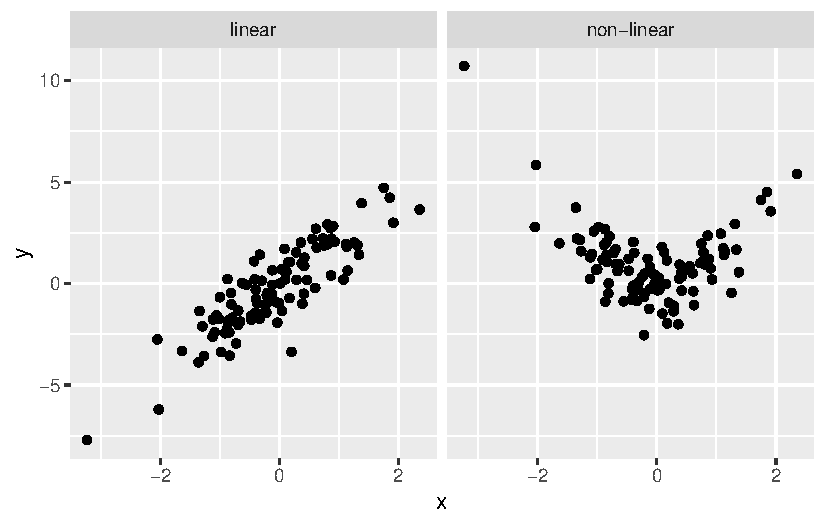
\includegraphics[keepaspectratio]{index_files/figure-pdf/unnamed-chunk-2-1.pdf}}

\begin{itemize}
\tightlist
\item
  方向：正相关vs负相关
\end{itemize}

\pandocbounded{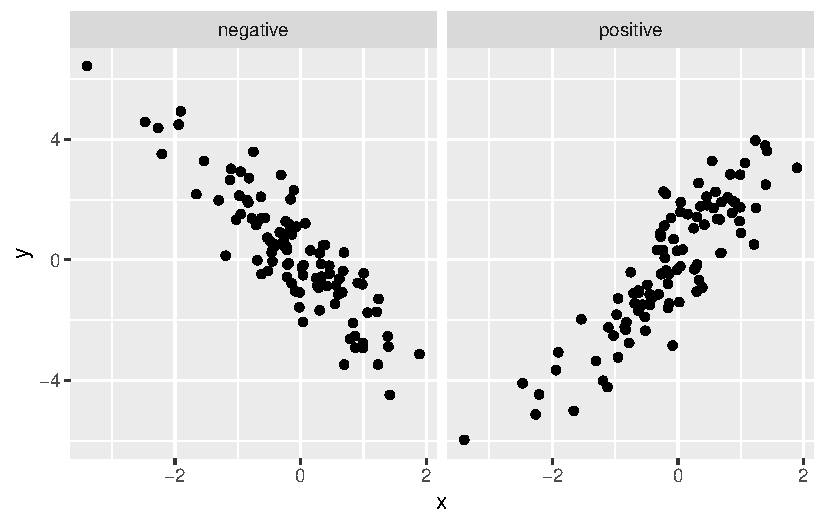
\includegraphics[keepaspectratio]{index_files/figure-pdf/unnamed-chunk-3-1.pdf}}

\begin{itemize}
\tightlist
\item
  程度：强相关vs弱相关
\end{itemize}

\pandocbounded{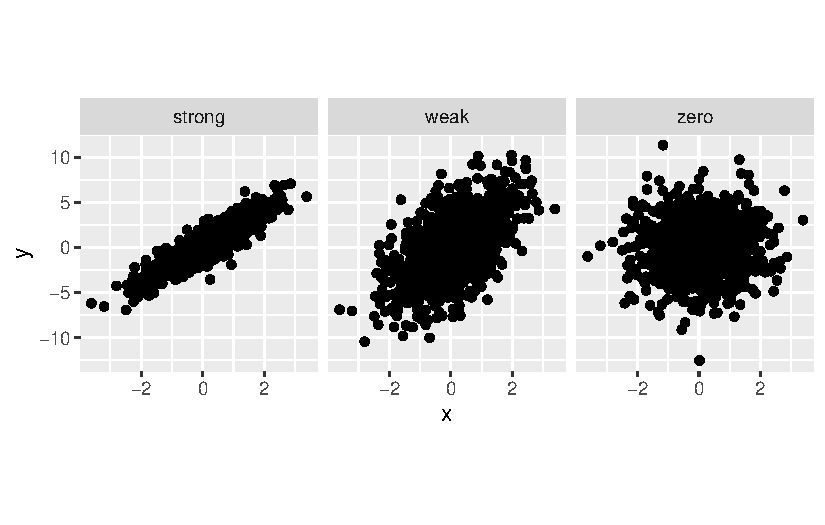
\includegraphics[keepaspectratio]{index_files/figure-pdf/unnamed-chunk-4-1.pdf}}

\section{皮尔逊相关系数}\label{ux76aeux5c14ux900aux76f8ux5173ux7cfbux6570}

皮尔逊相关系数的公式：

\begin{align}
SS_X &= \sum{(X-\bar{X})^2} \\
S_X^2 &= \frac{SS_X}{n-1} \\
Cov(X,Y) &= \frac{\sum(X-\bar{X})(Y-\bar{Y})}{n-1} \\
r_{XY} &= \frac{Cov(X,Y)}{S_XS_Y}
\end{align}

\section{皮尔逊相关分析的显著性检验}\label{ux76aeux5c14ux900aux76f8ux5173ux5206ux6790ux7684ux663eux8457ux6027ux68c0ux9a8c}

一般使用t检验对相关系数的显著性进行检验。

提出假设：

\begin{itemize}
\tightlist
\item
  H0: X与Y不相关（即，X与Y的相关为0）。
\item
  H1: X与Y相关（即，X与Y的相关不为0）。
\end{itemize}

皮尔逊相关系数的显著性检验本质上是将样本的相关系数r与虚无假设的0进行比较。

皮尔逊相关系数t检验中的标准误：

\begin{align}
SE &= \sqrt{\frac{1-r^2}{n-2}} \\
t &= \frac{r-0}{SE} \\
&= \frac{r}{SE} 
\end{align}

\begin{tcolorbox}[enhanced jigsaw, arc=.35mm, bottomrule=.15mm, bottomtitle=1mm, breakable, colback=white, colbacktitle=quarto-callout-caution-color!10!white, colframe=quarto-callout-caution-color-frame, coltitle=black, left=2mm, leftrule=.75mm, opacityback=0, opacitybacktitle=0.6, rightrule=.15mm, title=\textcolor{quarto-callout-caution-color}{\faFire}\hspace{0.5em}{注意}, titlerule=0mm, toprule=.15mm, toptitle=1mm]

相关系数的显著性只受样本量的影响，不受变量单位的影响。

\end{tcolorbox}

检验皮尔逊相关系数显著性的第二种方法是使用Fisher
z转换，本文对此不作介绍。

\section{皮尔逊相关分析}\label{ux76aeux5c14ux900aux76f8ux5173ux5206ux6790}

三种应对方式与抑郁的相关。

基于R base：

\begin{Shaded}
\begin{Highlighting}[numbers=left,,]
\NormalTok{vs }\OtherTok{\textless{}{-}} \FunctionTok{c}\NormalTok{(}\StringTok{"cope\_task1"}\NormalTok{, }\StringTok{"cope\_task2"}\NormalTok{, }\StringTok{"cope\_task3"}\NormalTok{, }
        \StringTok{"cope\_emo1"}\NormalTok{, }\StringTok{"cope\_emo2"}\NormalTok{, }\StringTok{"cope\_emo3"}\NormalTok{, }
        \StringTok{"cope\_avo1"}\NormalTok{, }\StringTok{"cope\_avo2"}\NormalTok{, }\StringTok{"cope\_avo3"}\NormalTok{, }
        \StringTok{"depr1"}\NormalTok{, }\StringTok{"depr2"}\NormalTok{, }\StringTok{"depr3"}\NormalTok{)}
\FunctionTok{round}\NormalTok{(}\FunctionTok{cov}\NormalTok{(depress[vs]), }\DecValTok{2}\NormalTok{)}
\DocumentationTok{\#\#            cope\_task1 cope\_task2 cope\_task3 cope\_emo1 cope\_emo2 cope\_emo3}
\DocumentationTok{\#\# cope\_task1         NA         NA         NA        NA        NA        NA}
\DocumentationTok{\#\# cope\_task2         NA         NA         NA        NA        NA        NA}
\DocumentationTok{\#\# cope\_task3         NA         NA         NA        NA        NA        NA}
\DocumentationTok{\#\# cope\_emo1          NA         NA         NA        NA        NA        NA}
\DocumentationTok{\#\# cope\_emo2          NA         NA         NA        NA        NA        NA}
\DocumentationTok{\#\# cope\_emo3          NA         NA         NA        NA        NA        NA}
\DocumentationTok{\#\# cope\_avo1          NA         NA         NA        NA        NA        NA}
\DocumentationTok{\#\# cope\_avo2          NA         NA         NA        NA        NA        NA}
\DocumentationTok{\#\# cope\_avo3          NA         NA         NA        NA        NA        NA}
\DocumentationTok{\#\# depr1              NA         NA         NA        NA        NA        NA}
\DocumentationTok{\#\# depr2              NA         NA         NA        NA        NA        NA}
\DocumentationTok{\#\# depr3              NA         NA         NA        NA        NA        NA}
\DocumentationTok{\#\#            cope\_avo1 cope\_avo2 cope\_avo3 depr1 depr2 depr3}
\DocumentationTok{\#\# cope\_task1        NA        NA        NA    NA    NA    NA}
\DocumentationTok{\#\# cope\_task2        NA        NA        NA    NA    NA    NA}
\DocumentationTok{\#\# cope\_task3        NA        NA        NA    NA    NA    NA}
\DocumentationTok{\#\# cope\_emo1         NA        NA        NA    NA    NA    NA}
\DocumentationTok{\#\# cope\_emo2         NA        NA        NA    NA    NA    NA}
\DocumentationTok{\#\# cope\_emo3         NA        NA        NA    NA    NA    NA}
\DocumentationTok{\#\# cope\_avo1         NA        NA        NA    NA    NA    NA}
\DocumentationTok{\#\# cope\_avo2         NA        NA        NA    NA    NA    NA}
\DocumentationTok{\#\# cope\_avo3         NA        NA        NA    NA    NA    NA}
\DocumentationTok{\#\# depr1             NA        NA        NA    NA    NA    NA}
\DocumentationTok{\#\# depr2             NA        NA        NA    NA    NA    NA}
\DocumentationTok{\#\# depr3             NA        NA        NA    NA    NA    NA}
\FunctionTok{round}\NormalTok{(}\FunctionTok{cor}\NormalTok{(depress[vs]), }\DecValTok{2}\NormalTok{)}
\DocumentationTok{\#\#            cope\_task1 cope\_task2 cope\_task3 cope\_emo1 cope\_emo2 cope\_emo3}
\DocumentationTok{\#\# cope\_task1          1         NA         NA        NA        NA        NA}
\DocumentationTok{\#\# cope\_task2         NA          1         NA        NA        NA        NA}
\DocumentationTok{\#\# cope\_task3         NA         NA          1        NA        NA        NA}
\DocumentationTok{\#\# cope\_emo1          NA         NA         NA         1        NA        NA}
\DocumentationTok{\#\# cope\_emo2          NA         NA         NA        NA         1        NA}
\DocumentationTok{\#\# cope\_emo3          NA         NA         NA        NA        NA         1}
\DocumentationTok{\#\# cope\_avo1          NA         NA         NA        NA        NA        NA}
\DocumentationTok{\#\# cope\_avo2          NA         NA         NA        NA        NA        NA}
\DocumentationTok{\#\# cope\_avo3          NA         NA         NA        NA        NA        NA}
\DocumentationTok{\#\# depr1              NA         NA         NA        NA        NA        NA}
\DocumentationTok{\#\# depr2              NA         NA         NA        NA        NA        NA}
\DocumentationTok{\#\# depr3              NA         NA         NA        NA        NA        NA}
\DocumentationTok{\#\#            cope\_avo1 cope\_avo2 cope\_avo3 depr1 depr2 depr3}
\DocumentationTok{\#\# cope\_task1        NA        NA        NA    NA    NA    NA}
\DocumentationTok{\#\# cope\_task2        NA        NA        NA    NA    NA    NA}
\DocumentationTok{\#\# cope\_task3        NA        NA        NA    NA    NA    NA}
\DocumentationTok{\#\# cope\_emo1         NA        NA        NA    NA    NA    NA}
\DocumentationTok{\#\# cope\_emo2         NA        NA        NA    NA    NA    NA}
\DocumentationTok{\#\# cope\_emo3         NA        NA        NA    NA    NA    NA}
\DocumentationTok{\#\# cope\_avo1          1        NA        NA    NA    NA    NA}
\DocumentationTok{\#\# cope\_avo2         NA         1        NA    NA    NA    NA}
\DocumentationTok{\#\# cope\_avo3         NA        NA         1    NA    NA    NA}
\DocumentationTok{\#\# depr1             NA        NA        NA     1    NA    NA}
\DocumentationTok{\#\# depr2             NA        NA        NA    NA     1    NA}
\DocumentationTok{\#\# depr3             NA        NA        NA    NA    NA     1}
\FunctionTok{cor.test}\NormalTok{(depress}\SpecialCharTok{$}\NormalTok{cope\_task1, depress}\SpecialCharTok{$}\NormalTok{depr1)}
\DocumentationTok{\#\# }
\DocumentationTok{\#\#  Pearson\textquotesingle{}s product{-}moment correlation}
\DocumentationTok{\#\# }
\DocumentationTok{\#\# data:  depress$cope\_task1 and depress$depr1}
\DocumentationTok{\#\# t = {-}5.9738, df = 172, p{-}value = 1.298e{-}08}
\DocumentationTok{\#\# alternative hypothesis: true correlation is not equal to 0}
\DocumentationTok{\#\# 95 percent confidence interval:}
\DocumentationTok{\#\#  {-}0.5305701 {-}0.2832149}
\DocumentationTok{\#\# sample estimates:}
\DocumentationTok{\#\#        cor }
\DocumentationTok{\#\# {-}0.4145194}
\end{Highlighting}
\end{Shaded}

基于\texttt{psych}程序包作相关矩阵热力图：

\begin{Shaded}
\begin{Highlighting}[numbers=left,,]
\FunctionTok{corPlot}\NormalTok{(depress[vs])}
\end{Highlighting}
\end{Shaded}

\begin{figure}[H]

{\centering \pandocbounded{
\includegraphics[keepaspectratio]{../../courses/PsyEduStat/correlation/cors.png}}

}

\caption{相关矩阵热力图}

\end{figure}%

基于\texttt{psych}程序包进行相关分析：

\begin{Shaded}
\begin{Highlighting}[numbers=left,,]
\CommentTok{\# test}
\NormalTok{out }\OtherTok{\textless{}{-}} \FunctionTok{corr.test}\NormalTok{(depress[vs])}
\NormalTok{out}
\DocumentationTok{\#\# Call:corr.test(x = depress[vs])}
\DocumentationTok{\#\# Correlation matrix }
\DocumentationTok{\#\#            cope\_task1 cope\_task2 cope\_task3 cope\_emo1 cope\_emo2 cope\_emo3}
\DocumentationTok{\#\# cope\_task1       1.00       0.63       0.45     {-}0.12     {-}0.14     {-}0.17}
\DocumentationTok{\#\# cope\_task2       0.63       1.00       0.76     {-}0.03      0.00     {-}0.04}
\DocumentationTok{\#\# cope\_task3       0.45       0.76       1.00     {-}0.06      0.00      0.05}
\DocumentationTok{\#\# cope\_emo1       {-}0.12      {-}0.03      {-}0.06      1.00      0.74      0.67}
\DocumentationTok{\#\# cope\_emo2       {-}0.14       0.00       0.00      0.74      1.00      0.81}
\DocumentationTok{\#\# cope\_emo3       {-}0.17      {-}0.04       0.05      0.67      0.81      1.00}
\DocumentationTok{\#\# cope\_avo1        0.02       0.04       0.06      0.27      0.28      0.22}
\DocumentationTok{\#\# cope\_avo2        0.07       0.11       0.02      0.10      0.21      0.17}
\DocumentationTok{\#\# cope\_avo3       {-}0.03      {-}0.03       0.06      0.16      0.28      0.28}
\DocumentationTok{\#\# depr1           {-}0.41      {-}0.26      {-}0.21      0.41      0.38      0.42}
\DocumentationTok{\#\# depr2           {-}0.28      {-}0.36      {-}0.32      0.42      0.48      0.54}
\DocumentationTok{\#\# depr3           {-}0.27      {-}0.32      {-}0.31      0.37      0.43      0.55}
\DocumentationTok{\#\#            cope\_avo1 cope\_avo2 cope\_avo3 depr1 depr2 depr3}
\DocumentationTok{\#\# cope\_task1      0.02      0.07     {-}0.03 {-}0.41 {-}0.28 {-}0.27}
\DocumentationTok{\#\# cope\_task2      0.04      0.11     {-}0.03 {-}0.26 {-}0.36 {-}0.32}
\DocumentationTok{\#\# cope\_task3      0.06      0.02      0.06 {-}0.21 {-}0.32 {-}0.31}
\DocumentationTok{\#\# cope\_emo1       0.27      0.10      0.16  0.41  0.42  0.37}
\DocumentationTok{\#\# cope\_emo2       0.28      0.21      0.28  0.38  0.48  0.43}
\DocumentationTok{\#\# cope\_emo3       0.22      0.17      0.28  0.42  0.54  0.55}
\DocumentationTok{\#\# cope\_avo1       1.00      0.66      0.57 {-}0.05 {-}0.03 {-}0.01}
\DocumentationTok{\#\# cope\_avo2       0.66      1.00      0.78 {-}0.09 {-}0.06 {-}0.05}
\DocumentationTok{\#\# cope\_avo3       0.57      0.78      1.00  0.03  0.07  0.06}
\DocumentationTok{\#\# depr1          {-}0.05     {-}0.09      0.03  1.00  0.67  0.64}
\DocumentationTok{\#\# depr2          {-}0.03     {-}0.06      0.07  0.67  1.00  0.81}
\DocumentationTok{\#\# depr3          {-}0.01     {-}0.05      0.06  0.64  0.81  1.00}
\DocumentationTok{\#\# Sample Size }
\DocumentationTok{\#\#            cope\_task1 cope\_task2 cope\_task3 cope\_emo1 cope\_emo2 cope\_emo3}
\DocumentationTok{\#\# cope\_task1        174        168        162       174       168       162}
\DocumentationTok{\#\# cope\_task2        168        173        166       168       173       166}
\DocumentationTok{\#\# cope\_task3        162        166        172       162       166       172}
\DocumentationTok{\#\# cope\_emo1         174        168        162       174       168       162}
\DocumentationTok{\#\# cope\_emo2         168        173        166       168       173       166}
\DocumentationTok{\#\# cope\_emo3         162        166        172       162       166       172}
\DocumentationTok{\#\# cope\_avo1         174        168        162       174       168       162}
\DocumentationTok{\#\# cope\_avo2         168        173        166       168       173       166}
\DocumentationTok{\#\# cope\_avo3         162        166        172       162       166       172}
\DocumentationTok{\#\# depr1             174        168        162       174       168       162}
\DocumentationTok{\#\# depr2             168        173        166       168       173       166}
\DocumentationTok{\#\# depr3             162        166        172       162       166       172}
\DocumentationTok{\#\#            cope\_avo1 cope\_avo2 cope\_avo3 depr1 depr2 depr3}
\DocumentationTok{\#\# cope\_task1       174       168       162   174   168   162}
\DocumentationTok{\#\# cope\_task2       168       173       166   168   173   166}
\DocumentationTok{\#\# cope\_task3       162       166       172   162   166   172}
\DocumentationTok{\#\# cope\_emo1        174       168       162   174   168   162}
\DocumentationTok{\#\# cope\_emo2        168       173       166   168   173   166}
\DocumentationTok{\#\# cope\_emo3        162       166       172   162   166   172}
\DocumentationTok{\#\# cope\_avo1        174       168       162   174   168   162}
\DocumentationTok{\#\# cope\_avo2        168       173       166   168   173   166}
\DocumentationTok{\#\# cope\_avo3        162       166       172   162   166   172}
\DocumentationTok{\#\# depr1            174       168       162   174   168   162}
\DocumentationTok{\#\# depr2            168       173       166   168   173   166}
\DocumentationTok{\#\# depr3            162       166       172   162   166   172}
\DocumentationTok{\#\# Probability values (Entries above the diagonal are adjusted for multiple tests.) }
\DocumentationTok{\#\#            cope\_task1 cope\_task2 cope\_task3 cope\_emo1 cope\_emo2 cope\_emo3}
\DocumentationTok{\#\# cope\_task1       0.00       0.00       0.00      1.00      1.00      0.98}
\DocumentationTok{\#\# cope\_task2       0.00       0.00       0.00      1.00      1.00      1.00}
\DocumentationTok{\#\# cope\_task3       0.00       0.00       0.00      1.00      1.00      1.00}
\DocumentationTok{\#\# cope\_emo1        0.11       0.69       0.49      0.00      0.00      0.00}
\DocumentationTok{\#\# cope\_emo2        0.06       0.98       0.98      0.00      0.00      0.00}
\DocumentationTok{\#\# cope\_emo3        0.03       0.59       0.52      0.00      0.00      0.00}
\DocumentationTok{\#\# cope\_avo1        0.83       0.57       0.46      0.00      0.00      0.01}
\DocumentationTok{\#\# cope\_avo2        0.39       0.14       0.77      0.18      0.01      0.03}
\DocumentationTok{\#\# cope\_avo3        0.75       0.70       0.47      0.04      0.00      0.00}
\DocumentationTok{\#\# depr1            0.00       0.00       0.01      0.00      0.00      0.00}
\DocumentationTok{\#\# depr2            0.00       0.00       0.00      0.00      0.00      0.00}
\DocumentationTok{\#\# depr3            0.00       0.00       0.00      0.00      0.00      0.00}
\DocumentationTok{\#\#            cope\_avo1 cope\_avo2 cope\_avo3 depr1 depr2 depr3}
\DocumentationTok{\#\# cope\_task1      1.00      1.00      1.00  0.00  0.01  0.02}
\DocumentationTok{\#\# cope\_task2      1.00      1.00      1.00  0.02  0.00  0.00}
\DocumentationTok{\#\# cope\_task3      1.00      1.00      1.00  0.25  0.00  0.00}
\DocumentationTok{\#\# cope\_emo1       0.01      1.00      1.00  0.00  0.00  0.00}
\DocumentationTok{\#\# cope\_emo2       0.01      0.19      0.01  0.00  0.00  0.00}
\DocumentationTok{\#\# cope\_emo3       0.19      0.78      0.01  0.00  0.00  0.00}
\DocumentationTok{\#\# cope\_avo1       0.00      0.00      0.00  1.00  1.00  1.00}
\DocumentationTok{\#\# cope\_avo2       0.00      0.00      0.00  1.00  1.00  1.00}
\DocumentationTok{\#\# cope\_avo3       0.00      0.00      0.00  1.00  1.00  1.00}
\DocumentationTok{\#\# depr1           0.55      0.22      0.70  0.00  0.00  0.00}
\DocumentationTok{\#\# depr2           0.68      0.43      0.35  0.00  0.00  0.00}
\DocumentationTok{\#\# depr3           0.87      0.54      0.44  0.00  0.00  0.00}
\DocumentationTok{\#\# }
\DocumentationTok{\#\#  To see confidence intervals of the correlations, print with the short=FALSE option}
\CommentTok{\# 查看相关分析的结果里面有哪些内容}
\FunctionTok{names}\NormalTok{(out)}
\DocumentationTok{\#\#  [1] "r"      "n"      "t"      "p"      "p.adj"  "se"     "sef"    "adjust"}
\DocumentationTok{\#\#  [9] "sym"    "ci"     "ci2"    "ci.adj" "stars"  "Call"}
\CommentTok{\# 调用查看out中的stars}
\NormalTok{out}\SpecialCharTok{$}\NormalTok{stars}
\DocumentationTok{\#\#            cope\_task1 cope\_task2 cope\_task3 cope\_emo1 cope\_emo2 cope\_emo3}
\DocumentationTok{\#\# cope\_task1 "1***"     "0.63***"  "0.45***"  "{-}0.12 "  "{-}0.14 "  "{-}0.17 " }
\DocumentationTok{\#\# cope\_task2 "0.63***"  "1***"     "0.76***"  "{-}0.03 "  "0 "      "{-}0.04 " }
\DocumentationTok{\#\# cope\_task3 "0.45***"  "0.76***"  "1***"     "{-}0.06 "  "0 "      "0.05 "  }
\DocumentationTok{\#\# cope\_emo1  "{-}0.12 "   "{-}0.03 "   "{-}0.06 "   "1***"    "0.74***" "0.67***"}
\DocumentationTok{\#\# cope\_emo2  "{-}0.14 "   "0 "       "0 "       "0.74***" "1***"    "0.81***"}
\DocumentationTok{\#\# cope\_emo3  "{-}0.17*"   "{-}0.04 "   "0.05 "    "0.67***" "0.81***" "1***"   }
\DocumentationTok{\#\# cope\_avo1  "0.02 "    "0.04 "    "0.06 "    "0.27***" "0.28***" "0.22**" }
\DocumentationTok{\#\# cope\_avo2  "0.07 "    "0.11 "    "0.02 "    "0.1 "    "0.21**"  "0.17*"  }
\DocumentationTok{\#\# cope\_avo3  "{-}0.03 "   "{-}0.03 "   "0.06 "    "0.16*"   "0.28***" "0.28***"}
\DocumentationTok{\#\# depr1      "{-}0.41***" "{-}0.26***" "{-}0.21**"  "0.41***" "0.38***" "0.42***"}
\DocumentationTok{\#\# depr2      "{-}0.28***" "{-}0.36***" "{-}0.32***" "0.42***" "0.48***" "0.54***"}
\DocumentationTok{\#\# depr3      "{-}0.27***" "{-}0.32***" "{-}0.31***" "0.37***" "0.43***" "0.55***"}
\DocumentationTok{\#\#            cope\_avo1 cope\_avo2 cope\_avo3 depr1      depr2      depr3    }
\DocumentationTok{\#\# cope\_task1 "0.02 "   "0.07 "   "{-}0.03 "  "{-}0.41***" "{-}0.28*"   "{-}0.27*" }
\DocumentationTok{\#\# cope\_task2 "0.04 "   "0.11 "   "{-}0.03 "  "{-}0.26*"   "{-}0.36***" "{-}0.32**"}
\DocumentationTok{\#\# cope\_task3 "0.06 "   "0.02 "   "0.06 "   "{-}0.21 "   "{-}0.32**"  "{-}0.31**"}
\DocumentationTok{\#\# cope\_emo1  "0.27**"  "0.1 "    "0.16 "   "0.41***"  "0.42***"  "0.37***"}
\DocumentationTok{\#\# cope\_emo2  "0.28**"  "0.21 "   "0.28**"  "0.38***"  "0.48***"  "0.43***"}
\DocumentationTok{\#\# cope\_emo3  "0.22 "   "0.17 "   "0.28**"  "0.42***"  "0.54***"  "0.55***"}
\DocumentationTok{\#\# cope\_avo1  "1***"    "0.66***" "0.57***" "{-}0.05 "   "{-}0.03 "   "{-}0.01 " }
\DocumentationTok{\#\# cope\_avo2  "0.66***" "1***"    "0.78***" "{-}0.09 "   "{-}0.06 "   "{-}0.05 " }
\DocumentationTok{\#\# cope\_avo3  "0.57***" "0.78***" "1***"    "0.03 "    "0.07 "    "0.06 "  }
\DocumentationTok{\#\# depr1      "{-}0.05 "  "{-}0.09 "  "0.03 "   "1***"     "0.67***"  "0.64***"}
\DocumentationTok{\#\# depr2      "{-}0.03 "  "{-}0.06 "  "0.07 "   "0.67***"  "1***"     "0.81***"}
\DocumentationTok{\#\# depr3      "{-}0.01 "  "{-}0.05 "  "0.06 "   "0.64***"  "0.81***"  "1***"}
\CommentTok{\# 当数据有缺失值时，使用FIML处理缺失值，然后计算相关系数}
\FunctionTok{round}\NormalTok{(}\FunctionTok{corFiml}\NormalTok{(depress[vs]), }\DecValTok{2}\NormalTok{)}
\DocumentationTok{\#\#            cope\_task1 cope\_task2 cope\_task3 cope\_emo1 cope\_emo2 cope\_emo3}
\DocumentationTok{\#\# cope\_task1       1.00       0.65       0.49     {-}0.10     {-}0.10     {-}0.11}
\DocumentationTok{\#\# cope\_task2       0.65       1.00       0.77      0.01      0.02     {-}0.01}
\DocumentationTok{\#\# cope\_task3       0.49       0.77       1.00      0.00      0.03      0.07}
\DocumentationTok{\#\# cope\_emo1       {-}0.10       0.01       0.00      1.00      0.73      0.66}
\DocumentationTok{\#\# cope\_emo2       {-}0.10       0.02       0.03      0.73      1.00      0.81}
\DocumentationTok{\#\# cope\_emo3       {-}0.11      {-}0.01       0.07      0.66      0.81      1.00}
\DocumentationTok{\#\# cope\_avo1        0.05       0.10       0.13      0.28      0.29      0.22}
\DocumentationTok{\#\# cope\_avo2        0.11       0.13       0.06      0.12      0.21      0.16}
\DocumentationTok{\#\# cope\_avo3        0.03       0.01       0.07      0.16      0.27      0.27}
\DocumentationTok{\#\# depr1           {-}0.41      {-}0.26      {-}0.20      0.41      0.36      0.41}
\DocumentationTok{\#\# depr2           {-}0.28      {-}0.35      {-}0.30      0.41      0.47      0.53}
\DocumentationTok{\#\# depr3           {-}0.25      {-}0.30      {-}0.31      0.35      0.43      0.54}
\DocumentationTok{\#\#            cope\_avo1 cope\_avo2 cope\_avo3 depr1 depr2 depr3}
\DocumentationTok{\#\# cope\_task1      0.05      0.11      0.03 {-}0.41 {-}0.28 {-}0.25}
\DocumentationTok{\#\# cope\_task2      0.10      0.13      0.01 {-}0.26 {-}0.35 {-}0.30}
\DocumentationTok{\#\# cope\_task3      0.13      0.06      0.07 {-}0.20 {-}0.30 {-}0.31}
\DocumentationTok{\#\# cope\_emo1       0.28      0.12      0.16  0.41  0.41  0.35}
\DocumentationTok{\#\# cope\_emo2       0.29      0.21      0.27  0.36  0.47  0.43}
\DocumentationTok{\#\# cope\_emo3       0.22      0.16      0.27  0.41  0.53  0.54}
\DocumentationTok{\#\# cope\_avo1       1.00      0.67      0.58 {-}0.05 {-}0.05 {-}0.05}
\DocumentationTok{\#\# cope\_avo2       0.67      1.00      0.77 {-}0.11 {-}0.07 {-}0.07}
\DocumentationTok{\#\# cope\_avo3       0.58      0.77      1.00  0.00  0.05  0.04}
\DocumentationTok{\#\# depr1          {-}0.05     {-}0.11      0.00  1.00  0.67  0.63}
\DocumentationTok{\#\# depr2          {-}0.05     {-}0.07      0.05  0.67  1.00  0.81}
\DocumentationTok{\#\# depr3          {-}0.05     {-}0.07      0.04  0.63  0.81  1.00}
\end{Highlighting}
\end{Shaded}

使用Keng程序包计算r的临界值：

\begin{Shaded}
\begin{Highlighting}[numbers=left,,]
\CommentTok{\# 样本量}
\FunctionTok{nrow}\NormalTok{(depress)}
\DocumentationTok{\#\# [1] 185}
\CommentTok{\# 计算r的临界值}
\FunctionTok{cut\_r}\NormalTok{(}\AttributeTok{n =} \DecValTok{94}\NormalTok{)}
\DocumentationTok{\#\#          p         r}
\DocumentationTok{\#\# [1,] 0.100 0.1706900}
\DocumentationTok{\#\# [2,] 0.050 0.2027627}
\DocumentationTok{\#\# [3,] 0.010 0.2644668}
\DocumentationTok{\#\# [4,] 0.001 0.3340562}
\end{Highlighting}
\end{Shaded}

基于上面计算得到的临界值，我们可以对任意一个相关系数的显著性水平做出判断。例如，r
= 0.234，0.243介于0.2027627与0.2644668之间，因此可以得出，对于r =
0.234，其p值小于0.05、大于0.01。

全文到此结束。




\end{document}
